\begin{figure*}[ht]
    \centering
    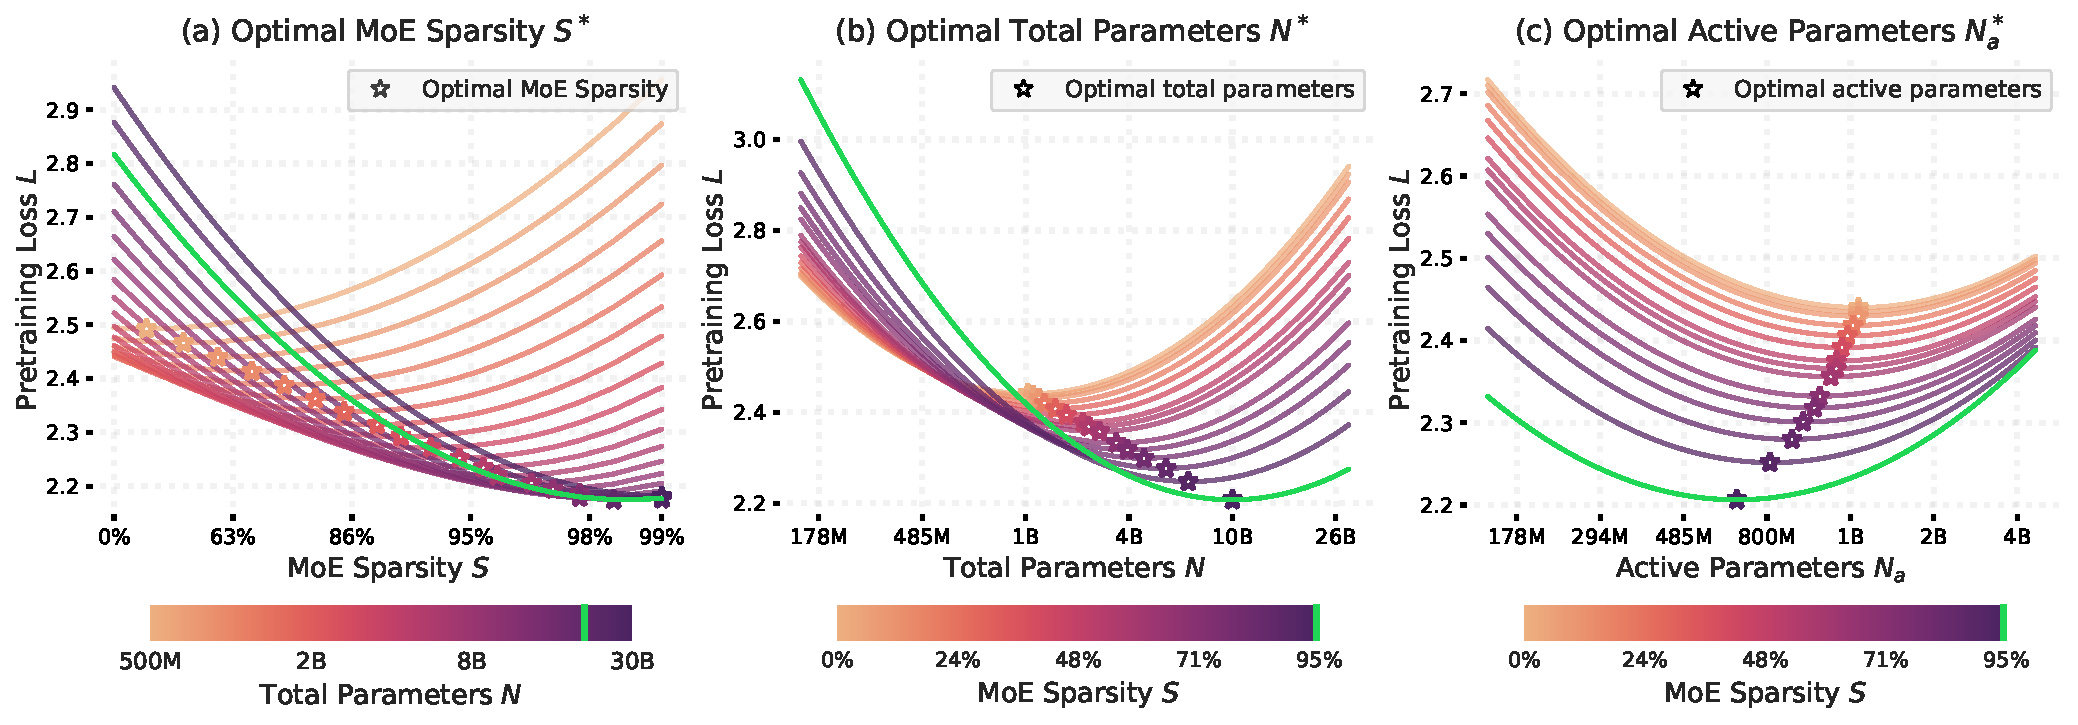
\includegraphics[width=0.95\textwidth]{plots/v2_s2_plot2_logS_colorbar_tickfix.pdf}
    \caption{\textbf{IsoFLOP slices along Sparsity and Model Size ($C=1e20$).}
    We use fitted isoFLOP surfaces (\Cref{sec:n_s_d_interaction}) to analyze how sparsity $\mathbf{S}$ and model size $\mathbf{N}$ impact the loss $\mathbf{L}$ for a fixed compute budget. We identify optimal points by (a) fixing $\mathbf{N}$ and varying $\mathbf{S}$, (b) fixing $\mathbf{S}$ and varying $\mathbf{N}$ and (c) fixing $\mathbf{S}$ and varying active parameters $\mathbf{N_a}$.  Observe that (a) the optimal sparsity $S$ increases with increasing model size $N$ and converges to 1 while (b) and (c) show that the optimal model size $N$ and active parameter count $N_a$ increase and decrease respectively with increasing sparsity levels. (see \Cref{fig:additional_surface_eval} in \Cref{app:n_s_d_interaction} for other total
training compute budgets.)
    \label{fig:iso_surface_sliced}
    }
\end{figure*}

\section{The Interplay between Model Parameters and Sparsity in \moes}
\label{sec:n_s_d_interaction}

Is there an optimal trade-off between parameter count and \flops per example in \moes under the setting where the training compute budget (i.e., total training \flops) is fixed?



Intuitively, under infinite data setting, scaling  model capacity along with the training compute budget leads to performance improvements. 
Previous scaling law studies suggest that, conditioned on a training compute budget measured in \flops denoted by \(C\), the optimal number of parameters, \(N^*(C)\), exhibits a power-law relationship with \(C\)~\citep{hoffmann2022training}:
\begin{equation}
    N^*(C) = \arg\min_{N} \mathcal{L}(N;C) \propto C^{a}
    \label{eqn:loss_n}
\end{equation}
Our goal is to study how to optimally trade-off \flops per example and total parameters in \moes.
In \moes the balance between parameters and \flops can be expressed through the sparsity level, $S$. We define $S$ as the ratio of non-active to total number of experts, i.e., $S = \frac{E - K}{E}$; where $E$ is the total number of experts and $K$ is the number of selected  experts per token. We can vary the sparsity level by either changing the number of active experts $K$ or total number of experts $E$.
\footnote{Sparsity level determines the number of active parameters given the total number of parameters and we use the active number of parameters as a proxy for \flops per example, as \( 6N_aD \) provides a good estimate of the total FLOP count for MoEs; see~\Cref{app:train_inference_cost} for details.}
Essentially, for models with the same \( N \), the model with a higher \( S \) will have fewer active parameters \( N_a \), resulting in fewer \flops per example. For more details on the notations and experimental settings see \Cref{app:prelim} and \Cref{app:exp_setup}.


\begin{equation}
    (N^*, S^*) = \arg\min_{N,S} \mathcal{L}(N,S;C)
    \label{eqn:optimal_ns_given_c}
\end{equation}

To simplify the problem of understanding the joint role of \( N \) and \( S \) in predicting \( L \), we break the problem, \Cref{eqn:optimal_ns_given_c}, into two parts:
\begin{enumerate}[left=0pt,itemsep=2pt]
\item \textit{"How does the sparsity level impact the scaling laws of the relationship between \( N \) and \( C \) for training-compute optimal models?"}
To address this question in \S\ref{sec:fix_sparsity_vary_params}, we fix \( S \) and vary \( N \), studying how optimal \( N \) and \( N_a \) change for different values of \( S \):
\begin{equation}
    N^* = \argmin_{N} \mathcal{L}(N; C, S)
\label{eq:fix_sparsity_vary_N}
\end{equation}
\item \textit{"Is there an optimal balance between total number of parameters and the sparsity level under fixed training-compute budget?"}
To address this question in \S\ref{sec:fix_params_vary_sparsity}, we fix \( N \) and vary \( S \), studying how optimal \( S \) changes across different values of \( N \):
\begin{equation}
    S^* = \argmin_{S} \mathcal{L}(S; C, N)
\label{eq:fix_N_vary_sparsity}
\end{equation}
\end{enumerate}
As the first step, considering a fixed training compute budget \( C \), we fit a 3D surface, referred to as the IsoFLOP surface, in \Cref{fig:iso_surface}a, using a polynomial function, following approach II of \citet{hoffmann2022training}. 
Compared to \citet{hoffmann2022training} we include the sparsity variable and fit a single 3d IsoFLOP surface across all data points, rather than fitting separate 2d IsoFLOP curves for fixed sparsity levels or model sizes. 
We conducted a grid search to determine the optimal polynomial degree for \( N \), \( S \), and the interaction term \( N \times S \), finding that a degree of \( (2, 2, 2) \) resulted in the lowest cross-validation error. Both \( N \) and \( S \) are in log space (see \Cref{app:exp_setup} for more details).

As seen in \Cref{fig:iso_surface}a, the IsoFLOP surface plot is parabolic along model size, suggesting that the findings of \citet{hoffmann2022training} extend to MoEs across different sparsity levels, i.e., \( \mathcal{L}(N; C, S) \) is parabolic, with its optimal solution located at the turning point. When considering the total number of parameters $N$, the optimal value increases as the sparsity level increases, while for the active number of parameters $N_a$ the optimal value decreases with the sparsity level. This indicates that by increasing the sparsity level the training compute optimal models are larger but have fewer \flops per example, i.e., lower inference cost. 
Moreover, along sparsity, the pretraining loss decreases monotonically, indicating that, for the same compute budget, sparser models achieve better pretraining performance. We observe the same pattern across different training compute budgets (See \Cref{app:n_s_d_interaction}). To better understand and explain these observations, we examine slices of the IsoFLOP surface along the axes of \( S \) and \( N \) separately in \S\ref{sec:fix_sparsity_vary_params} and \S\ref{sec:fix_params_vary_sparsity}, respectively.

\subsection{Optimal Model Size for Fixed Sparsity Level}
\label{sec:fix_sparsity_vary_params}

Here we examine how sparsity influences scaling laws governing the relationship between \( N \), \(N_a\) and \( C \) for training-compute optimal models, i.e. how does \( N^* \) and \( N_a^* \), for a given $C,S$ 
(\Cref{eq:fix_sparsity_vary_N}), change as we increase \( S \)?
Looking at slices of the IsoFLOP surface along the model size dimension, in \Cref{fig:iso_surface_sliced}b and \Cref{fig:iso_surface_sliced}c, we observe how the IsoFLOP curves shift along loss and model size. 
Considering the training-compute optimal model, for a fixed compute budget, loss decreases as we increase sparsity. Furthermore, while sparser models have larger \( N \) compared to denser models, as seen in \Cref{fig:iso_surface_sliced}b, they have a smaller active parameter count \( N_a \); hence, fewer FLOPs per example. Intuitively, more parameters in total increase the capacity of the sparser models to fit the data, while fewer number of active parametes, hence fewer \flops per example, allow the model to be trained with more tokens, i.e., higher \( D \), for the same training compute budget. 

\subsection{Optimal Sparsity Level for Fixed Model Size}
\label{sec:fix_params_vary_sparsity}
In this section we aim to understand the dynamics between the total number of parameters and \flops per example in \moes. 
In \Cref{sec:fix_sparsity_vary_params} we are considering the case where there is no bound on the total number of parameters. In this case, we observe that under fixed training  compute budget in terms of \flops, it is better to train  sparser models with higher total number of parameters. However in practical scenarios it is reasonable to assume that there would be some bounds on the memory and hence the total number of parameters of a model. 
This leads us to a fundamental question: Is there an optimal balance between the total number of parameters and and \flops per example under a fixed training-compute budget? 
Thus, we investigate the optimal sparsity level when total number of parameters is fixed.
Specifically, we ask: Given \(N\) and \(C\), How does \(S^*\) change as we vary \(N\)?

To address this, we look into slices of the IsoFLOP surface along the sparsity dimension. As we can see in \Cref{fig:iso_surface_sliced}a, for a fixed training compute budget and fixed model size $\mathcal{L}(S; N,C)$ exhibits a parabolic profile, reaching its optimum value at the vertex where $S = S^*$. It is noteworthy that for a given total training compute, there is threshold value $N_{th}$ for the total number of parameters, where for larger models, models with \( N > N_{th} \), increasing sparsity always has a positive impact, i.e., optimal sparsity level approaches $1.0$. More accurately, for a fixed compute budget the optimal sparsity level increases with model size and converges to $1$ as the model size grows (see \Cref{fig:opt_sparsity} in \S\ref{app:budget} in the Appendix for more details).
Note that the optimal model, here is not the largest model, i.e., there is a compute optimal model size in terms of total parameters even after sparsity is introduced, and increasing total number of parameters would lead to under-training if training compute budget is fixed.

These results highlight the importance of balancing the number of parameters with \flops per example in \moes. Intuitively, when the total number of parameters is small, higher sparsity results in fewer active parameters, and thus fewer \flops per example. This reduction in \flops per example may lead to inefficiencies during both training and inference. Conversely, when the total number of parameters is large, for a reasonable amount of \flops per example, a fixed compute budget may not allow sufficient training on enough tokens to make use of the model's additional capacity.
